\documentclass[unicode,11pt,a4paper,oneside,numbers=endperiod,openany]{scrartcl}

\usepackage{graphicx}
\usepackage{subcaption}
%\usepackage{auto-pst-pdf}

\usepackage{ifthen}
\usepackage[utf8]{inputenc}
\usepackage{graphics}
\usepackage{graphicx}
\usepackage{hyperref}

\pagestyle{plain}
\voffset -5mm
\oddsidemargin  0mm
\evensidemargin -11mm
\marginparwidth 2cm
\marginparsep 0pt
\topmargin 0mm
\headheight 0pt
\headsep 0pt
\topskip 0pt        
\textheight 255mm
\textwidth 165mm

\newcommand{\duedate} {}
\newcommand{\setduedate}[1]{%
\renewcommand\duedate {Due date:~ #1}}
\newcommand\isassignment {false}
\newcommand{\setassignment}{\renewcommand\isassignment {true}}
\newcommand{\ifassignment}[1]{\ifthenelse{\boolean{\isassignment}}{#1}{}}
\newcommand{\ifnotassignment}[1]{\ifthenelse{\boolean{\isassignment}}{}{#1}}

\newcommand{\assignmentpolicy}{
\begin{table}[h]
\begin{center}
\scalebox{0.8} {%
\begin{tabular}{|p{0.02cm}p{16cm}|}
\hline
&\\
\multicolumn{2}{|c|}{\Large\textbf{HPC Lab for CSE 2020 ---  Submission Instructions}}\\
\multicolumn{2}{|c|}{\large\textbf{(Please, notice that following instructions are mandatory: }}\\
\multicolumn{2}{|c|}{\large\textbf{submissions that don't comply with, won't be considered)}}\\
&\\
\textbullet & Assignments must be submitted to \href{https://moodle-app2.let.ethz.ch/course/view.php?id=12315}{Moodle} (i.e. in electronic format).\\
\textbullet & Provide both executable package and sources (e.g. C/C++ files, Matlab). 
If you are using libraries, please add them in the file. Sources must be organized in directories called:\\
\multicolumn{2}{|c|}{\textit{Project\_number\_lastname\_firstname}}\\
& and  the  file must be called:\\
\multicolumn{2}{|c|}{\textit{project\_number\_lastname\_firstname.zip}}\\
\multicolumn{2}{|c|}{\textit{project\_number\_lastname\_firstname.pdf}}\\
\textbullet &  The TAs will grade your project by reviewing your project write-up, and looking at the implementation 
                 you attempted, and benchmarking your code's performance.\\

\textbullet & You are allowed to discuss all questions with anyone you like; however: (i) your submission must list anyone you discussed problems with and (ii) you must write up your submission independently.\\
\hline
\end{tabular}
}
\end{center}
\end{table}
}
\newcommand{\punkte}[1]{\hspace{1ex}\emph{\mdseries\hfill(#1~\ifcase#1{Points}\or{Points}\else{Points}\fi)}}


\newcommand\serieheader[6]{
\thispagestyle{empty}%
\begin{flushleft}

\includegraphics[width=0.4\textwidth]{eth_logo_kurz_pos_13}
\end{flushleft}
  \noindent%
  {\large\ignorespaces{\textbf{#1}}\hspace{\fill}\ignorespaces{ \textbf{#2}}}\\ \\%
  {\large\ignorespaces #3 \hspace{\fill}\ignorespaces #4}\\
  \noindent%
  \bigskip
  \hrule\par\bigskip\noindent%
  \bigskip {\ignorespaces {\Large{\textbf{#5}}}
  \hspace{\fill}\ignorespaces \large \ifthenelse{\boolean{\isassignment}}{\duedate}{#6}}
  \hrule\par\bigskip\noindent%  \linebreak
 }

\makeatletter
\def\enumerateMod{\ifnum \@enumdepth >3 \@toodeep\else
      \advance\@enumdepth \@ne
      \edef\@enumctr{enum\romannumeral\the\@enumdepth}\list
      {\csname label\@enumctr\endcsname}{\usecounter
        {\@enumctr}%%%? the following differs from "enumerate"
	\topsep0pt%
	\partopsep0pt%
	\itemsep0pt%
	\def\makelabel##1{\hss\llap{##1}}}\fi}
\let\endenumerateMod =\endlist
\makeatother




\usepackage{textcomp}





\begin{document}


\setassignment
\setduedate{09.03.2020 (midnight)}

\serieheader{High-Performance Computing Lab for CSE}{2020}{Student: Sina Klampt}{Discussed with: Alain Hügli, Anna Hutter}{Solution for Project 1}{}
\newline

\assignmentpolicy
In this project you will practice memory access optimization, performance-oriented programming, and OpenMP parallelizaton 
on Euler.

\section{Explaining Memory Hierarchies \punkte{30}}

\subsection{Identifying Parameters}
Using the commands given on the exercise sheet, I was able to find the following values for the memory hierarchy on the computer node of the Euler cluster:
\begin{center}
    \begin{tabular}{ |l|l| }
    \hline
    Main memory & 32 GB \\ \hline
    L3 cache & 6 MB \\ \hline
    L2 cache & 256 kB \\ \hline
    L1 cache & 32 kB \\
    \hline
    \end{tabular}
\end{center}

\subsection{Running Membench}
In this exercise we were supposed to run the membench program on our local machine and on the Euler cluster.

The first plot (Fig. 1) represents the results on my local machine. I have a Intel Core i7 processor with 16 GB of Main Memory, 196 kB of L1 cache, 2 MB of L2 cache and 8 MB of L3 cache.

The second plot (Fig. 2) represents the results using Euler. I have used the Xeon Gold 6150 CPU.
When we look at the time axis, we can easily see that the performance of the Euler cluster is much better than on my local machine.
\begin{figure}[h!]
    \centering
    %\includegraphics[width=2]{generic.ps}
    \caption{Plot for local machine}
\end{figure}
\begin{figure}[h!]
    \centering
    %\includegraphics{./generic_euler.ps}
    \caption{Plot for Euler}
\end{figure}

\subsection{Memory Access Patterns}
In the first case we had: csize = 128 and stride = 1. Since one integer corresponds to 4 Bytes, we have 128 times 4 which equals 512. Thus we need to look at the red line corresponding to 0.5 kB.

In the second case we had: csize = $2^{20}$ and stride = csize/2. This time we get csize = $2^{22}$ Byte (4 MB) and stride = $2^{21}$ Byte (2 MB). Thus we have to look at the light blue line.

\subsection{Temporal Locality}
asdf


\section{Optimize Square Matrix-Matrix Multiplication  \punkte{70}}

\subsection{Optimizing Part One}

\subsection{Optimizing Part Two}

\end{document}
